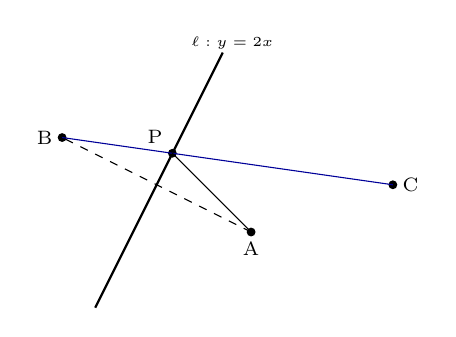
\begin{tikzpicture}[x=6mm,y=6mm]
\ax{-2}{7}{-0.6}{5}
\draw[thick,domain=-0.3:2.4,samples=80] plot (\x,{2*\x});
\fill (3,1) circle (1.6pt);
\node[below] at (3,1){\scriptsize A};
\fill (-1,3) circle (1.6pt);
\node[left] at (-1,3){\scriptsize B};
\fill (6,2) circle (1.6pt);
\node[right] at (6,2){\scriptsize C};
\fill (1.3333333333333333,2.6666666666666665) circle (1.6pt);
\node[above left] at (1.3333333333333333,2.6666666666666665){\scriptsize P};
\draw[dashed] (3,1)--(-1,3); \draw[blue!60!black] (-1,3)--(6,2); \draw (3,1)--(1.333,2.667); \node at (2.6,5){\tiny $\ell:y=2x$};
\end{tikzpicture}